\documentclass{beamer}

\mode<presentation>
{
  \useinnertheme[shadow=true]{rounded} % default from Warsaw theme
  \useoutertheme[subsection=false]{miniframes}

  \usecolortheme{orchid} % default from Warsaw theme
  \usecolortheme{whale} % default from Warsaw theme
  \usecolortheme{beaver} % this overrides both orchid and whale, as far as I~see, but keep them for safety

  % these override \usecolortheme above
  \setbeamercolor{frametitle}{bg=,fg=darkred!80!black}
  \setbeamercolor{frametitle right}{bg=}
  \setbeamercolor{palette tertiary}{fg=black,bg=gray!15!white}

  \usefonttheme[onlylarge]{structurebold}
  \setbeamerfont{block title}{size={}} % default from Warsaw theme
  \setbeamerfont{frametitle}{series=\bfseries} % probably taken care of by structurebold anyway, but keep in case useful for the future

  \setbeamercovered{transparent}
}

\usepackage[polish]{babel}
\usepackage[utf8]{inputenc}
\usepackage{times}
\usepackage[T1]{fontenc}

\title{Compositing Shaders in~X3D}
\author[Michalis Kamburelis]{Michalis Kamburelis \\ \texttt{michalis.kambi@gmail.com}}
\institute{Institute of Computer Science\\ University of Wroc{\l}aw, Poland}
\date{TPCG 2011}

\AtBeginSection[]
{
  \begin{frame}<beamer>{Outline}
    \tableofcontents[currentsection,currentsubsection]
  \end{frame}
}

\begin{document}

{
  % logo
  \pgfdeclareimage[height=4cm]{ii-and-kambivrml}{ii-and-kambivrml}
  \logo{\pgfuseimage{ii-and-kambivrml}}

  % Use background on title slide only,
  % trick from http://www.tug.org/pipermail/texhax/2007-March/008035.html
%  \usebackgroundtemplate{
\includegraphics[width=\paperwidth]{bg-lighter}}
  \begin{frame}
    \titlepage
  \end{frame}
}

\begin{frame}{Outline}
  \tableofcontents
  % You might wish to add the option [pausesections]
\end{frame}

\section{Introduction}

\begin{frame}{Introduction}
How to create and composite powerful graphic effects using shaders.

\begin{itemize}
  \item Extension of two existing languages (X3D and~GLSL).
  \item Practical, implemented (100\% finished open-source
    implementation).
\end{itemize}
\end{frame}

\begin{frame}{Easy and~works}

Easy, but no-one else did it before :)

\begin{itemize}
  \item Actually there are other systems trying to achieve this by inventing
    completely new languages (Spark, Sh). They necessarily sit on top
    of existing languages like GLSL. Using them is quite involved,
    as you don't want to implement a new shader language yourself.
    So practically you have to make a renderer specifically targeted
    at a given language and it's single implementation (like libsh).

  \item  We propose much simpler approach, no new language, just a natural
    extension for X3D and GLSL (or other shading language, actually, like Cg).
    % Should be easy to implement if you already have X3D browser.
\end{itemize}

Works perfectly :) Various shading algorithms become easy to implement,
and the implementation is automatically reusable.
No need to reimplement your shaders for each scene/configuration.

    % Istotnie pozwalam na~programowanie i~łączenie efektów
    % za~pomocą shaderów w~bardzo wygodny sposób.
    %  IMHO dopiero teraz GLSL jest użyteczny dla~autorów.

\end{frame}

\section{What is X3D, what are shaders}

\begin{frame}[fragile]{X3D}

\begin{itemize}
  \item \textbf{Extensible 3D}: language to describe 3D worlds.
  \item Open (full specifications on~\texttt{http://www.web3d.org/}), popular standard.
  \item Easy to express all typical 3D world features.
  \item In simple cases, a tree of nodes.
    In a general case, a directed graph of nodes, cycles possible.
  \item Each node has a set of fields, some fields contain in turn children nodes.
\end{itemize}

\begin{exampleblock}{Example}
\begin{semiverbatim}
\#X3D V3.2 utf8
PROFILE Interchange
Shape \{
  geometry Sphere \{ radius 2 \}
\}
\end{semiverbatim}
\end{exampleblock}
\end{frame}

\begin{frame}[fragile]{X3D - XML}

Alternative example:

\begin{exampleblock}{Example encoded in XML}
\begin{semiverbatim}
...
<X3D version="3.2" profile="Interchange" ...>
  <Scene>
    <Shape>
      <Sphere radius="2" />
    </Shape>
  </Scene>
</X3D>
\end{semiverbatim}
\end{exampleblock}

\end{frame}

% TODO- remove, instead more slides about our invention?
\begin{frame}{X3D as a programming language}

There are some aspects of X3D that make it more interesting,
more like ``(declarative) programming language'' than just ``3D model format'':

\begin{itemize}
  \item DEF/USE: references, for all nodes.
  \item Events: sending and receiving events,
    declarative analogy to calling a method in imperative programming.
    E.g.~open a door when user presses a handled.
  \item Prototypes: define new nodes,
  %pełnowartościowe,
    by combining existing ones.
  \item Scripts: integration with script languages (like JavaScript) easy.
    Script remains a ,,black box'' for~X3D, and at the same time
    in X3D we define exactly what parts of the scene are accessed.
     %  np.~JavaScript. U mnie --- z~własnym prostym językiem skryptowym
     % oraz ze skompilowanym kodem w~ObjectPascalu.
     % Więcej nowinek w~vrml\_engine\_doc, sekcja "advanced features".
\end{itemize}
\end{frame}

\begin{frame}{Shaders}
Shaders:
\begin{itemize}
  \item Languages to calculate color of 3D shapes. Implement per-vertex work,
    let GPU rasterize, implement per-pixel (fragment) work.
    % Chociaż przy pomocy pewnych sztuczek (tekstury oparte na~float,
    % render to textury) można je wykorzystać do~ogólnych obliczeń,
    % obecnie do~ogólnych obliczeń wygodniejsze są CUDA/OpenCL
    % (google.com/q=gpgpu).
    % Można próbować
    % geom shader
  \item We focus on real-time GPU shaders here.
    Popular choices: GLSL (OpenGL), Cg (NVidia: OpenGL or Direct 3D),
    HLSL (Direct 3D).
  \item Of course, you can use shaders in X3D.
\end{itemize}
\end{frame}

\begin{frame}[fragile]
\begin{exampleblock}{Example X3D + GLSL}
\begin{semiverbatim}
\#X3D V3.2 utf8
PROFILE Interchange
Shape \{
  appearance Appearance \{
    shaders ComposedShader \{
      language "GLSL"
      parts ShaderPart \{
        type "FRAGMENT"
        url "data:text/plain,
        \textbf{void main(void)}
        \textbf{\{}
          \textbf{gl\_FragColor = vec4(1.0,0.0,0.0,1.0);}
        \textbf{\}}" \} \} \}
  geometry Sphere \{ radius 2 \}
\}
\end{semiverbatim}
\end{exampleblock}
\end{frame}

\begin{frame}{Shader replaces the calculations}

\begin{itemize}
  %  \item + Wybiera pierwszy obsługiwany shader.
  %% \item + Można łatwo przekazać do~shadera wartości uniform (per-object)
  %%   albo attribute (per-vertex). Np.~przekaż aktualny czas
  %%    to shadera.
  \item + Easy implementation for renderer, since this is how GPU works,
    this is what OpenGL exposes etc.
  \item - \textbf{Difficult implementation of your own shaders}.
    Before implementing your effects, first learn to recreate
    the necessary features from fixed-function.
    Sure, you can let some renderer auto-generate a large shader for you,
    and only modify it, but...
  \item - \textbf{You create one-time shaders, not reusable}.
    Particular shader is tied to scene configuration (lights and textures
    counts, types etc.). General shader implementing everything
    would be awfully slow, unless you use \texttt{\#ifdefs} --- in which case
    it's awfully large.
  \item - \textbf{All the effects in one huge shader}.
    Ultimately, following this means you create a large shader,
    that is not maintainable. Adding / removing an effect means carefully
    inserting logic into a large code.
\end{itemize}
\end{frame}

\section[Our idea]{Our idea: compositing shaders in X3D}

\begin{frame}{Why}
\begin{itemize}
  \item We would like to intensively use shaders. Every 3D property
    should be programmable --- that's the reason why shaders were created.

  \item Traditional approach, ``write shader that does everything'',
    makes it difficult to actually harness that power.
    Implementing a simplest change (like ``filter light through a stencil'')
    requires understanding and taking care of the algorithm around.

  \item We prefer to create effects that extend/modify existing behaviors.
\end{itemize}
\end{frame}

\begin{frame}{Solution}

\begin{block}{Idea 1}
Easy to use mechanism to define and~use
``sockets'' (plugs) --- places where you can insert your own calculations.
To use a socket named \texttt{texture\_apply},
just define (in GLSL) function with a magic name \texttt{PLUG\_texture\_apply}
in a new node \texttt{Effect}.
\end{block}

\begin{itemize}
  \item We keep the full power of the shading language (GLSL).
    %% - You still have the full power of shading language like GLSL
    %%   (we do~not hide it from you, we do~not invent any new language
    %%   for writing shaders, and implementation doesn't have to do~any
    %%   difficult operations to process your shading language code).
  \item Implementation in~renderer easy: we extend existing language.
  \item Implementation of new effects easy: implement
    your desired effect, only point our how it is tied to the existing
    calculations.
  \item Effects are reusable: inserted into an internal shader,
    optimized for particular textures, lights etc.
  \item Effects can be composited: multiple effects may refer to the same sockets.
\end{itemize}
\end{frame}

\begin{frame}[fragile]
\begin{exampleblock}{Example of our effect}
\begin{semiverbatim}
# inside an Appearance node from previous example:
effects Effect \{
  language "GLSL"
  parts EffectPart \{
    type "FRAGMENT"
    url "data:text/plain,
\textbf{    void PLUG\_texture\_apply(}
\textbf{      inout vec4 fragment\_color,}
\textbf{      const in vec3 normal)}
\textbf{    \{}
\textbf{      fragment\_color.rgb *= 2.0;}
\textbf{    \}}"
  \}
\}
\end{semiverbatim}
\end{exampleblock}
\end{frame}

%\renewcommand*{\figurename}{Obraz}

\begin{frame}{Details}
\begin{itemize}
  \item New node \texttt{Effect}: choose shading language, like GLSL.
  \item New node \texttt{EffectPart}: choose type (vertex, pixel, etc.).
  \item You can define new uniform values in an~\texttt{Effect} node,
    for example pass a texture or current time (\texttt{TimeSensor.time} in~X3D)
    to the effect.
    % jak ComposedShader
  \item All effects are added to the base internal shader. (Oversimplifying a little.)
  \item Old \texttt{ComposedShader} node modifies the base shader.
    This way old, standard \texttt{ComposedShader} node becomes more powerful too:
    it can cooperate with internal effects (like shadow maps),
    and~user effects (from \texttt{Effect} nodes).
\end{itemize}
\end{frame}

\begin{frame}{Example - compositing two trivial effects}
\begin{figure}
  \centering
  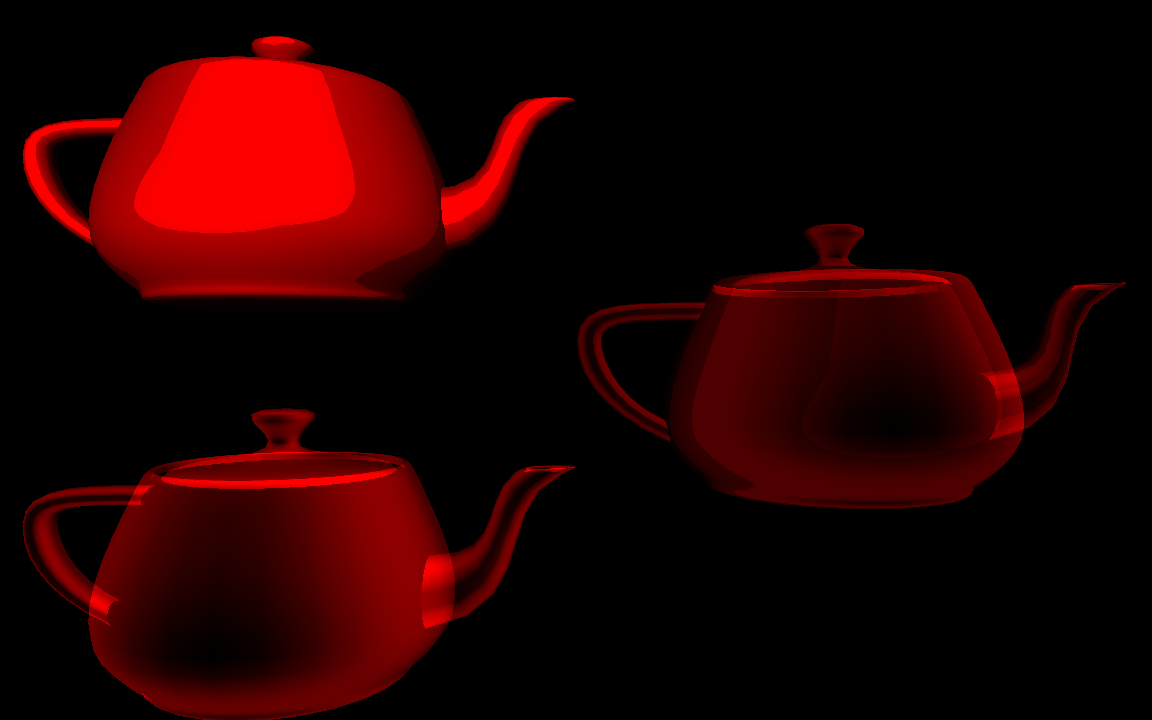
\includegraphics[width=3.0in]{../fresnel_and_toon}
  \caption{Composite Fresnel effect and~toon shading}
\end{figure}

Code: \texttt{demo\_models/compositing\_shaders/\\fresnel\_and\_toon.x3dv}

  %% : show the X3D source:
  %%   I~can just say: "this is a list of effects you should use:
  %%   this one, and this one. Now make it happen."
  %%   And both effects are applied.
\end{frame}

\begin{frame}{Internal effects}
Renderer can implement internal effects in a similar way.
This is invisible to user, and allows for really nice orthogonal implementation
of some features:

\begin{itemize}
  \item Shadow maps: filter particular light source,
  \item Classic Bump mapping: change normal vector based on texture value.
  \item Fog: mix final color with a fog color.
\end{itemize}

\begin{figure}
  \centering
  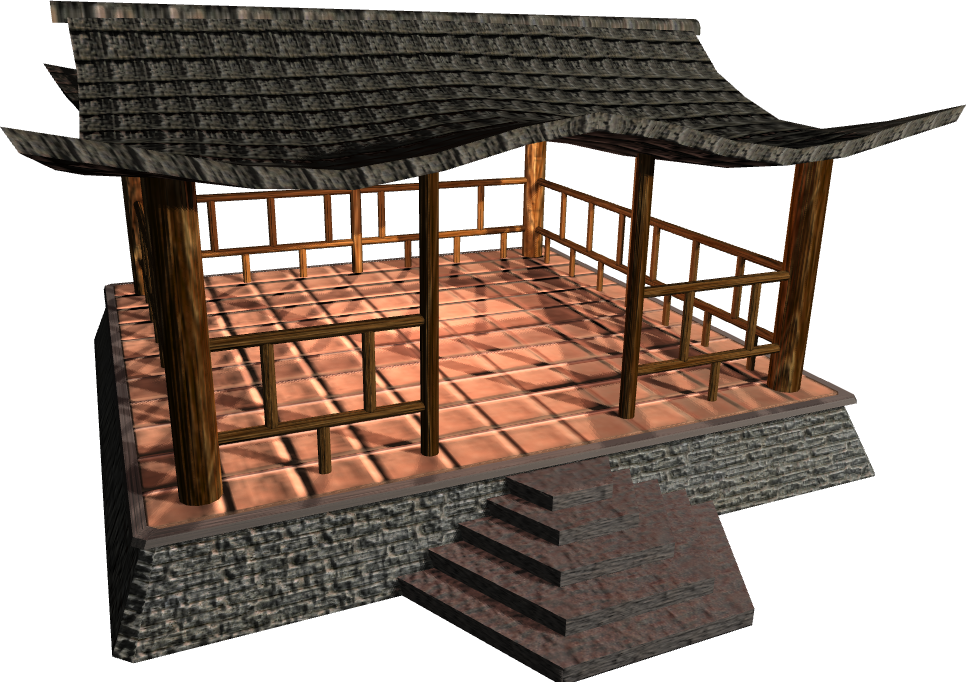
\includegraphics[width=2in]{../rhan_shrine_5_everything}
  \caption{Compositing two shadow maps and~bump mapping}
\end{figure}
\end{frame}

\begin{frame}{Light sources effects}
\begin{block}{Idea 2}
Effects may be added not only to visible 3D shapes.
Also lights can have their own effects, that gives that a specific
shape, equation etc. Such light becomes a fully-fledged, reusable X3D
light source.
\end{block}

\begin{figure}
  \centering
  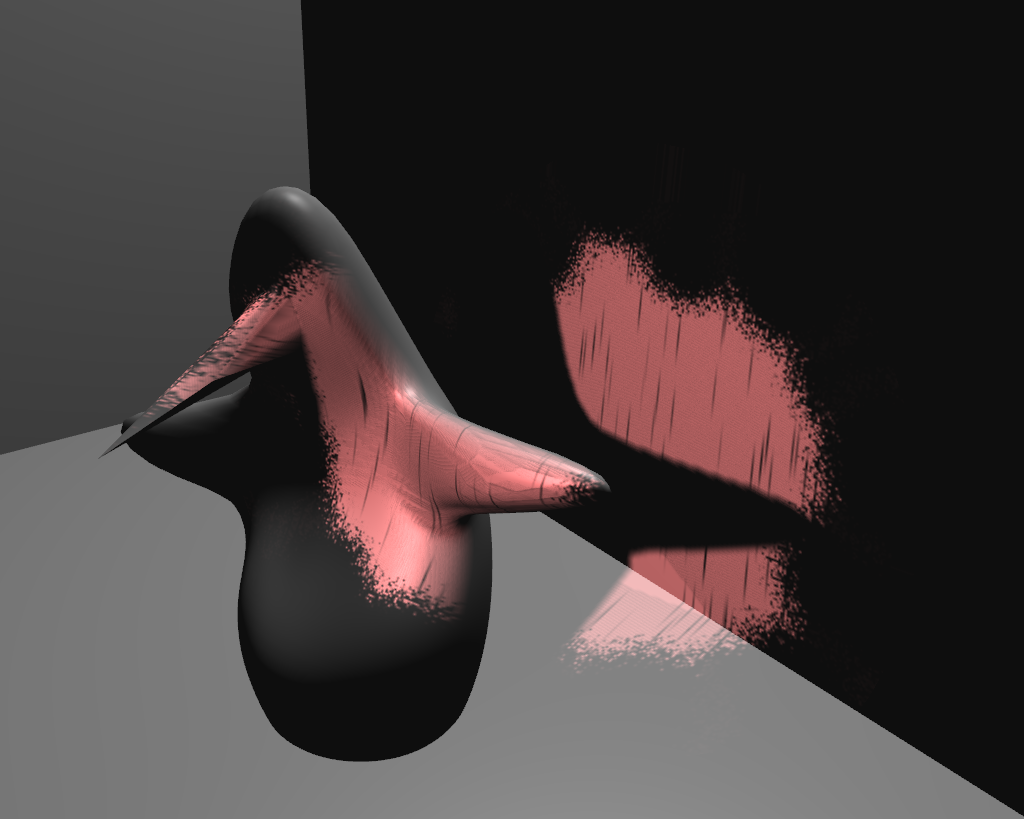
\includegraphics[width=1.8in]{../fancy_light_spot_shape}
  \caption{Light filtered through a texture. Casts a proper shape, cooperates with~bump mapping (which doesn't occur with simple texture projection), without any work from author.}
\end{figure}
\end{frame}

\begin{frame}[fragile]{Texture effects}
Textures can naturally also be modified using the effects.
A lot of possibilities, as textures are just 2D and 3D containers for general data
in many algorithms.

\vspace{0.1in}

E.g.~add noise to existing texture, or choose a 2D slice of 3D texture.
\end{frame}

\begin{frame}[fragile]{Procedural textures on GPU}
Procedural texture is just a function 2D or~3D $\rightarrow$
color, normal vector, and~such.

\vspace{0.1in}

Using procedural textures in shading languages was always possible,
but usual approaches have some quirks: since a procedural isn't a texture
in a usual sense (there is no related storage on GPU), usually it wasn't
easy to generate texture coordinates in a comfortable way for procedural
textures. We invent here \texttt{ShaderTexture} node, that is a really
nice way of expressing procedural textures calculated by GPU.

\begin{center}
\begin{columns}[T]
  \begin{column}{1in}
    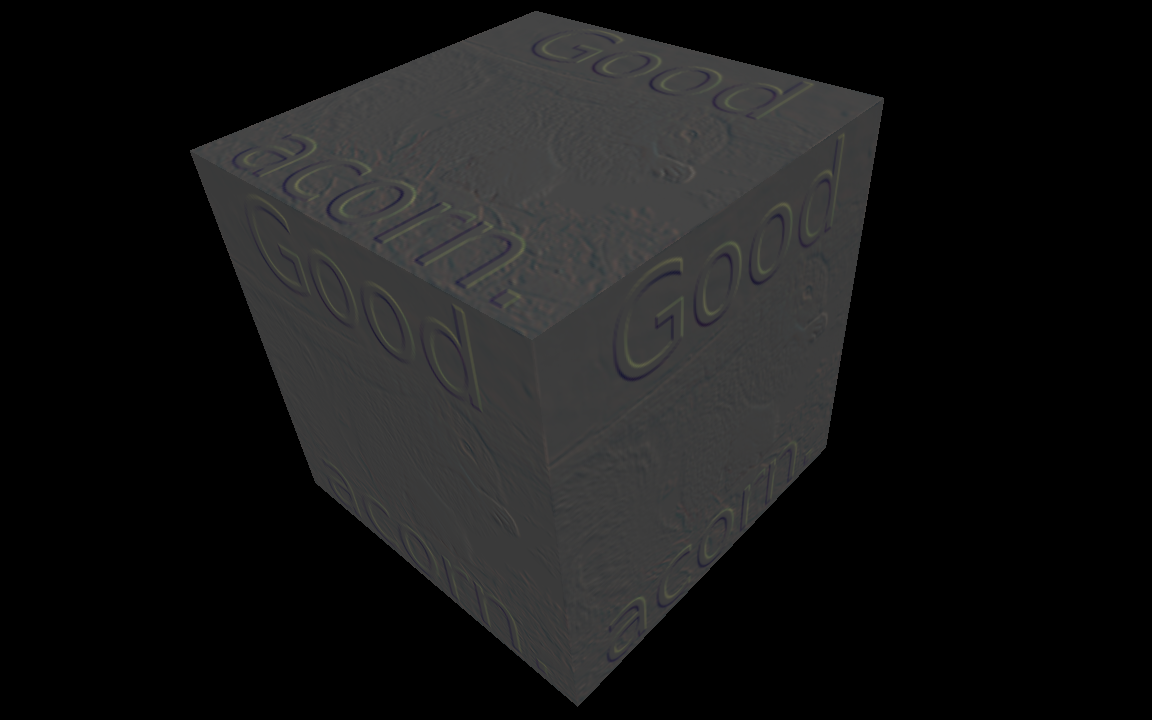
\includegraphics[width=1.3in]{../shader_texture_edge_detection}
  \end{column}
  \begin{column}{1in}
    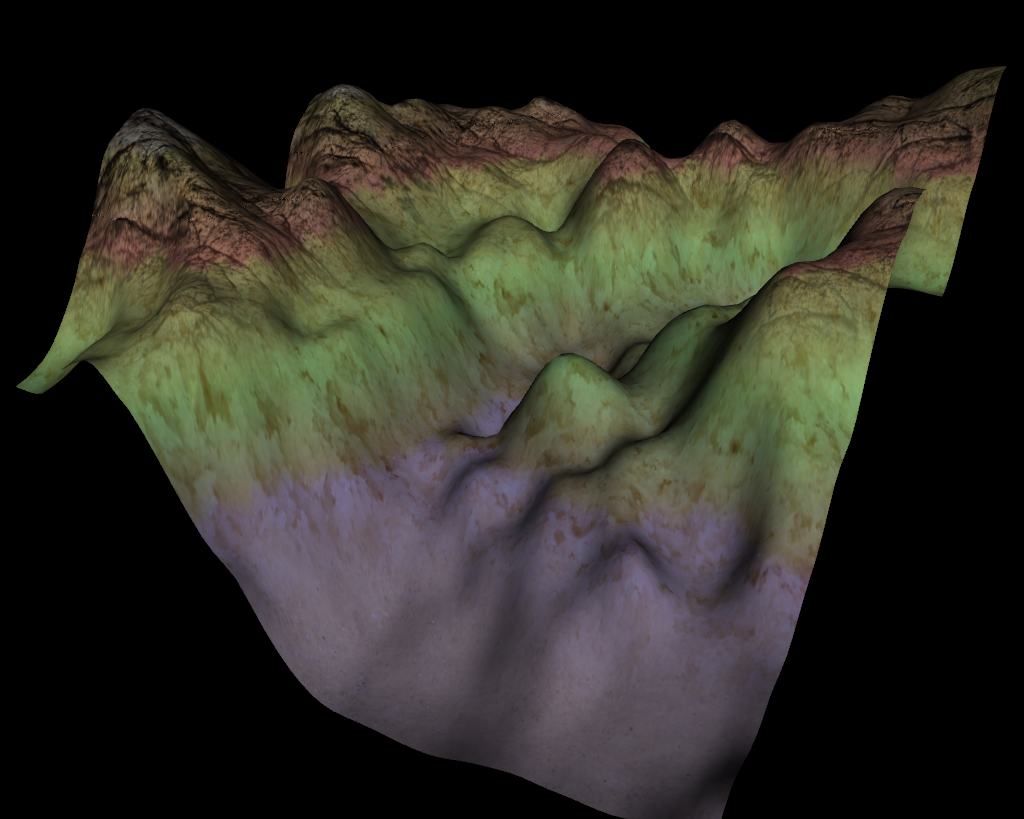
\includegraphics[width=1.3in]{../terrain}
  \end{column}
  \begin{column}{1in}
    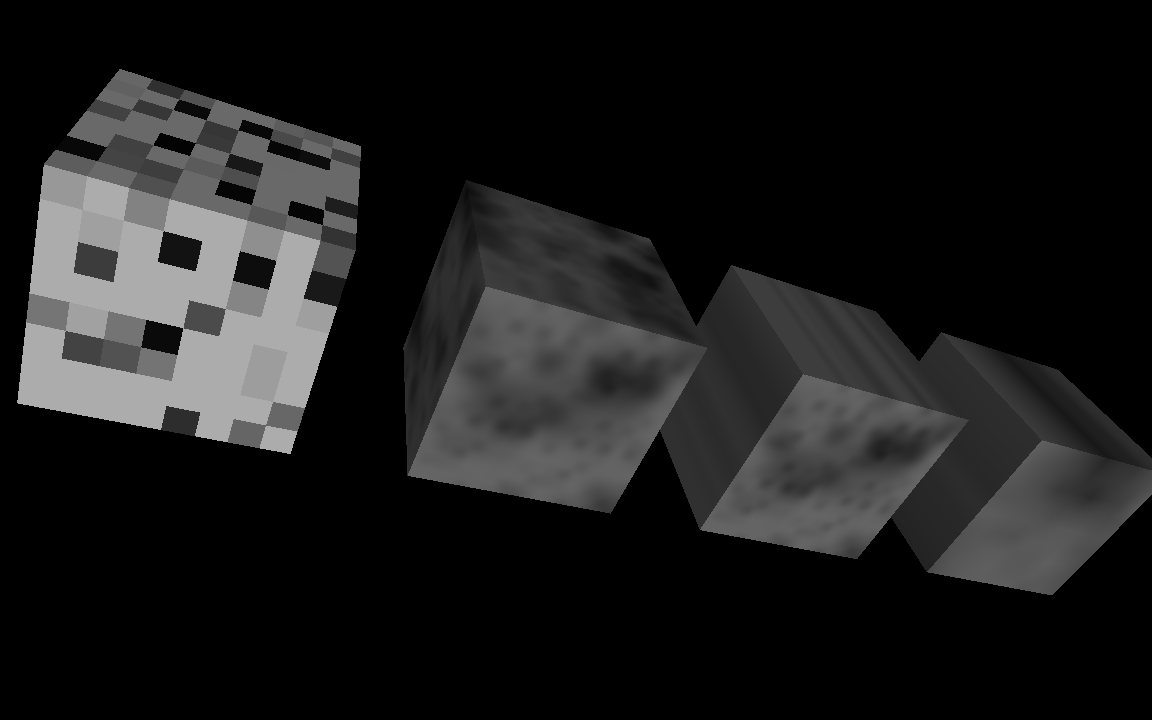
\includegraphics[width=1.3in]{../noise}
  \end{column}
\end{columns}
\end{center}

\end{frame}

\begin{frame}{Group effects}
%Naturalne rozszerzenie.

\begin{figure}
  \centering
  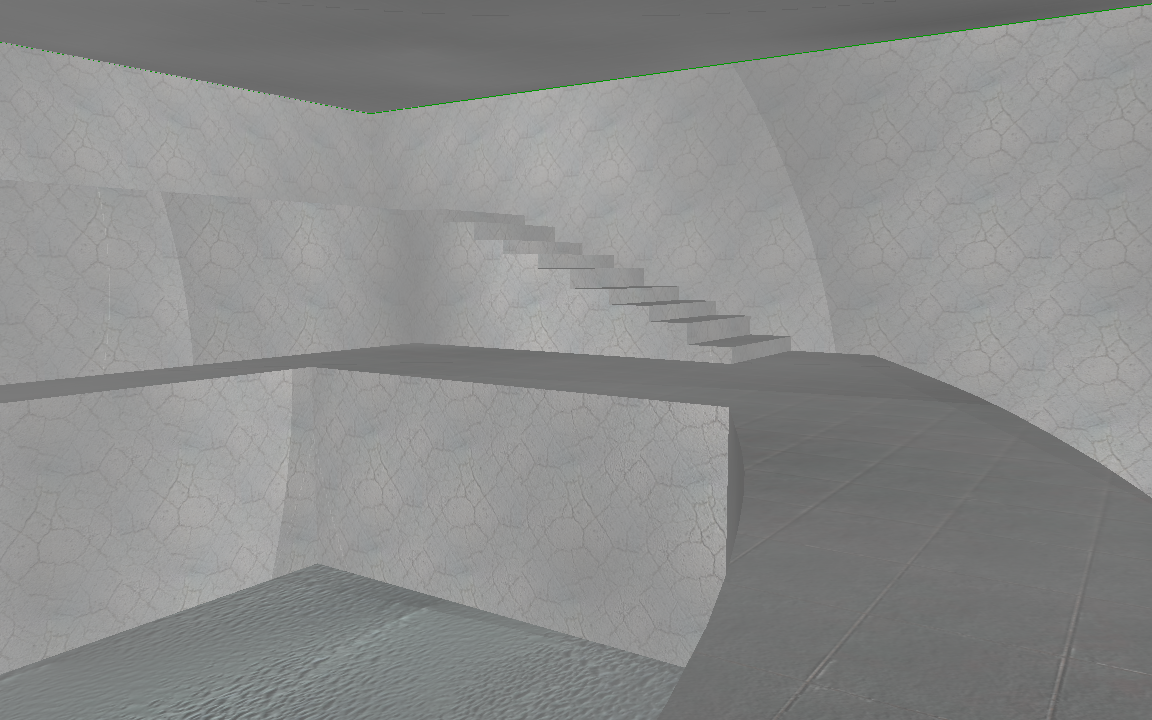
\includegraphics[width=3in]{../volumetric_animated_fog_all}
  \caption{Dense animated fog (sauna).}
\end{figure}

Code: \texttt{demo\_models/compositing\_shaders/\\volumetric\_animated\_fog.x3dv}\\
\textbf{Short and~works on~any 3D model!}

% Unline other implementation.)
% Turn on/off fog.

\end{frame}

\begin{frame}{Defining custom plugs}
You can easily define your own plugs (sockets) trivially easy:
\begin{itemize}
  \item Base shader, and \textbf{every effect}, can define plugs
    to be available for following effects.\\
    Just add a magic comment \texttt{/* PLUG: ... */} inside.
  \item Magic comment may be used multiple times (to enable loop
    unrolling in shaders, sometimes necessary).
  \item Magic comment \texttt{/* PLUG-DECLARATION */}
    (useful to declare GLSL version etc.).
  \item We nicely use the \textit{separate compilation units} of the GLSL.
  \item Idea portable to other shading languages.
  \item Good choice of default plugs, see links at the end.
    Despite our fear, it turns our that we don't need 100 plugs
    --- a couple of plugs fills the needs of 90\% of use cases.
\end{itemize}
\end{frame}

\begin{frame}{Final examples - water}
\begin{figure}
  \centering
  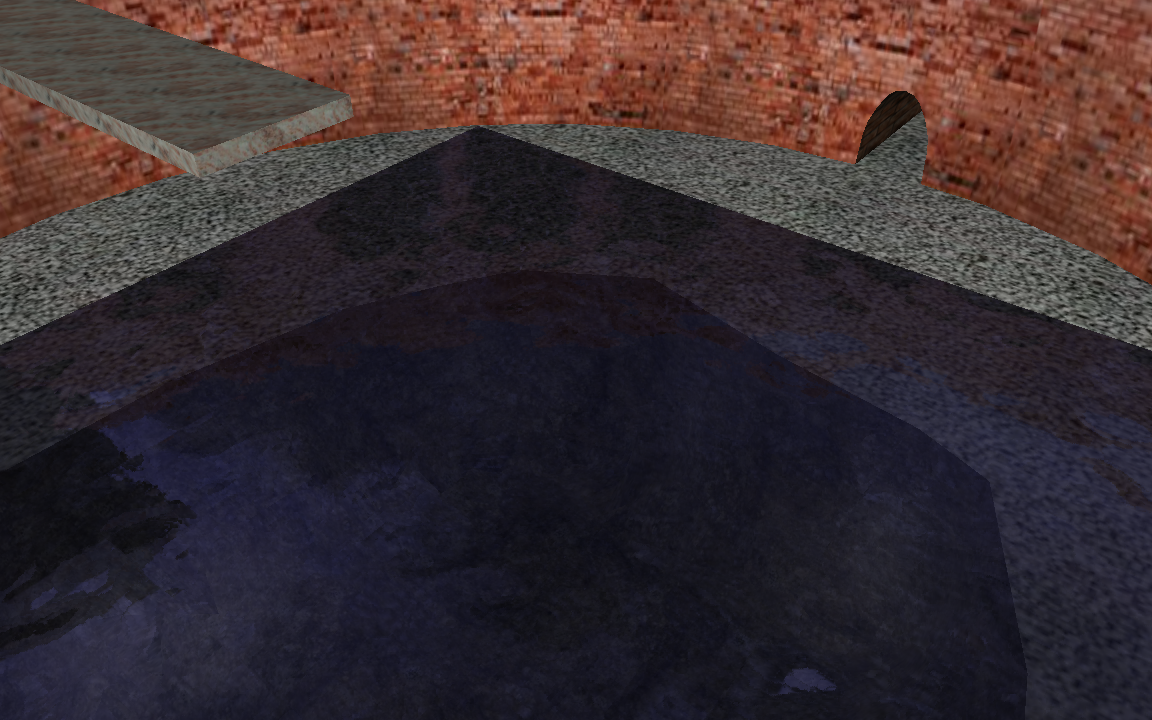
\includegraphics[width=3.5in]{../water_shaders_3}
  \caption{Water, combination of a couple of effects: generate normal vectors in tangent space, transform to eye space, mix with color from reflection and refraction.}
\end{figure}
\end{frame}

\begin{frame}
\begin{figure}
  \centering
  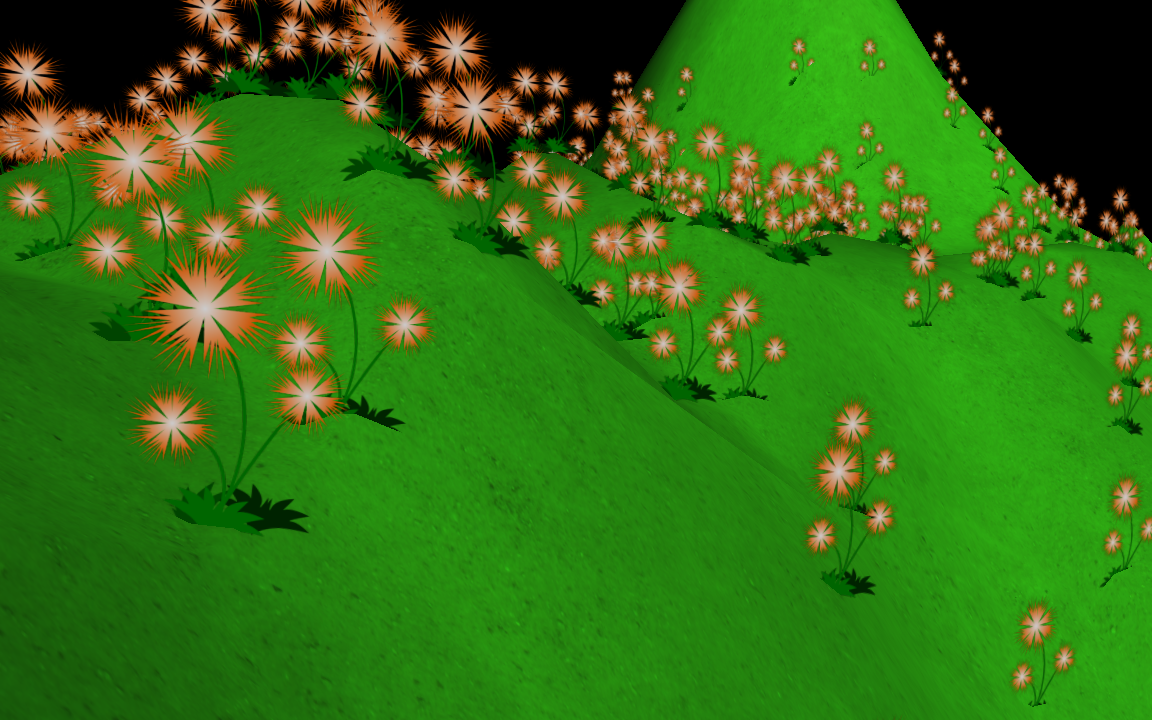
\includegraphics[width=3.5in]{../flowers}
  \caption{Animated flowers: transforming in object space by shaders, with zero speed cost.}
\end{figure}
\end{frame}

\section{Questions?}

\begin{frame}[t]

\begin{center}
{\small
Everything is implemented, open-source (LGPL), in~our engine:\\
{\color{blue} \textbf{\texttt{http://vrmlengine.sourceforge.net/}}}\\
Instructions how to download and view examples are here:\\
{\color{blue} \textbf{\texttt{http://vrmlengine.sourceforge.net/\\
compositing\_shaders.php}}}}
\end{center}

\vspace{0.25in}

\begin{center}
{\Large Thank you for your attention!}
\end{center}

%\vspace{0.1in}

\begin{center}
{\Huge \alert{Questions?}}
\end{center}

\end{frame}

\end{document}
